%!TeX root = ../main.tex

{\raggedright\large\textbf{Local feature compression using autoencoders - SfM tests}}\smallskip \\ 
Design a compression strategy for local SURF descriptors using autoencoders. Training data can be generated using the images of dataset Portello and Castle. Testing must be done on dataset FountainP-11 and Tiso (available at \url{https://github.com/openMVG/SfM_quality_evaluation/tree/master/Benchmarking_Camera_Calibration_2008} and \url{http://www.dei.unipd.it/~sim1mil/materiale/3Drecon/}). Software must be implemented in MATLAB, Keras or Pytorch. \\ \textbf{Testing on 3D reconstruction using SfM:} The reconstructed descriptors (only for the test set) are used to perform a SfM reconstruction using COLMAP (using the two test dataset). \\
Programming languages: MATLAB/Python/C++.

\section{Introduction}

The experiment was firstly performed by prof. Arecchi Fortunato around 1965 and it exhibits the difference between a coherent and a thermal source. Despite the important results, the setup is quite straightforward: it consists in a laser source, an \emph{Arecchi wheel} (a reflecting sandpaper planar wheel) and a photodetector capable of collecting light via a single-mode fiber. The laser source shines on the \emph{Arecchi wheel} and reflects inside the photodetector. If the wheel is still then the photodetector ``sees'' a coherent light source, while if it is spinning then a thermal source is simulated, because of the multiple reflections from the rough surface of the sandpaper. In figure \ref{fig:setup} the setup of the experiment is graphically represented.

% Insert images like this:
\begin{figure}[h!]
    \centering
    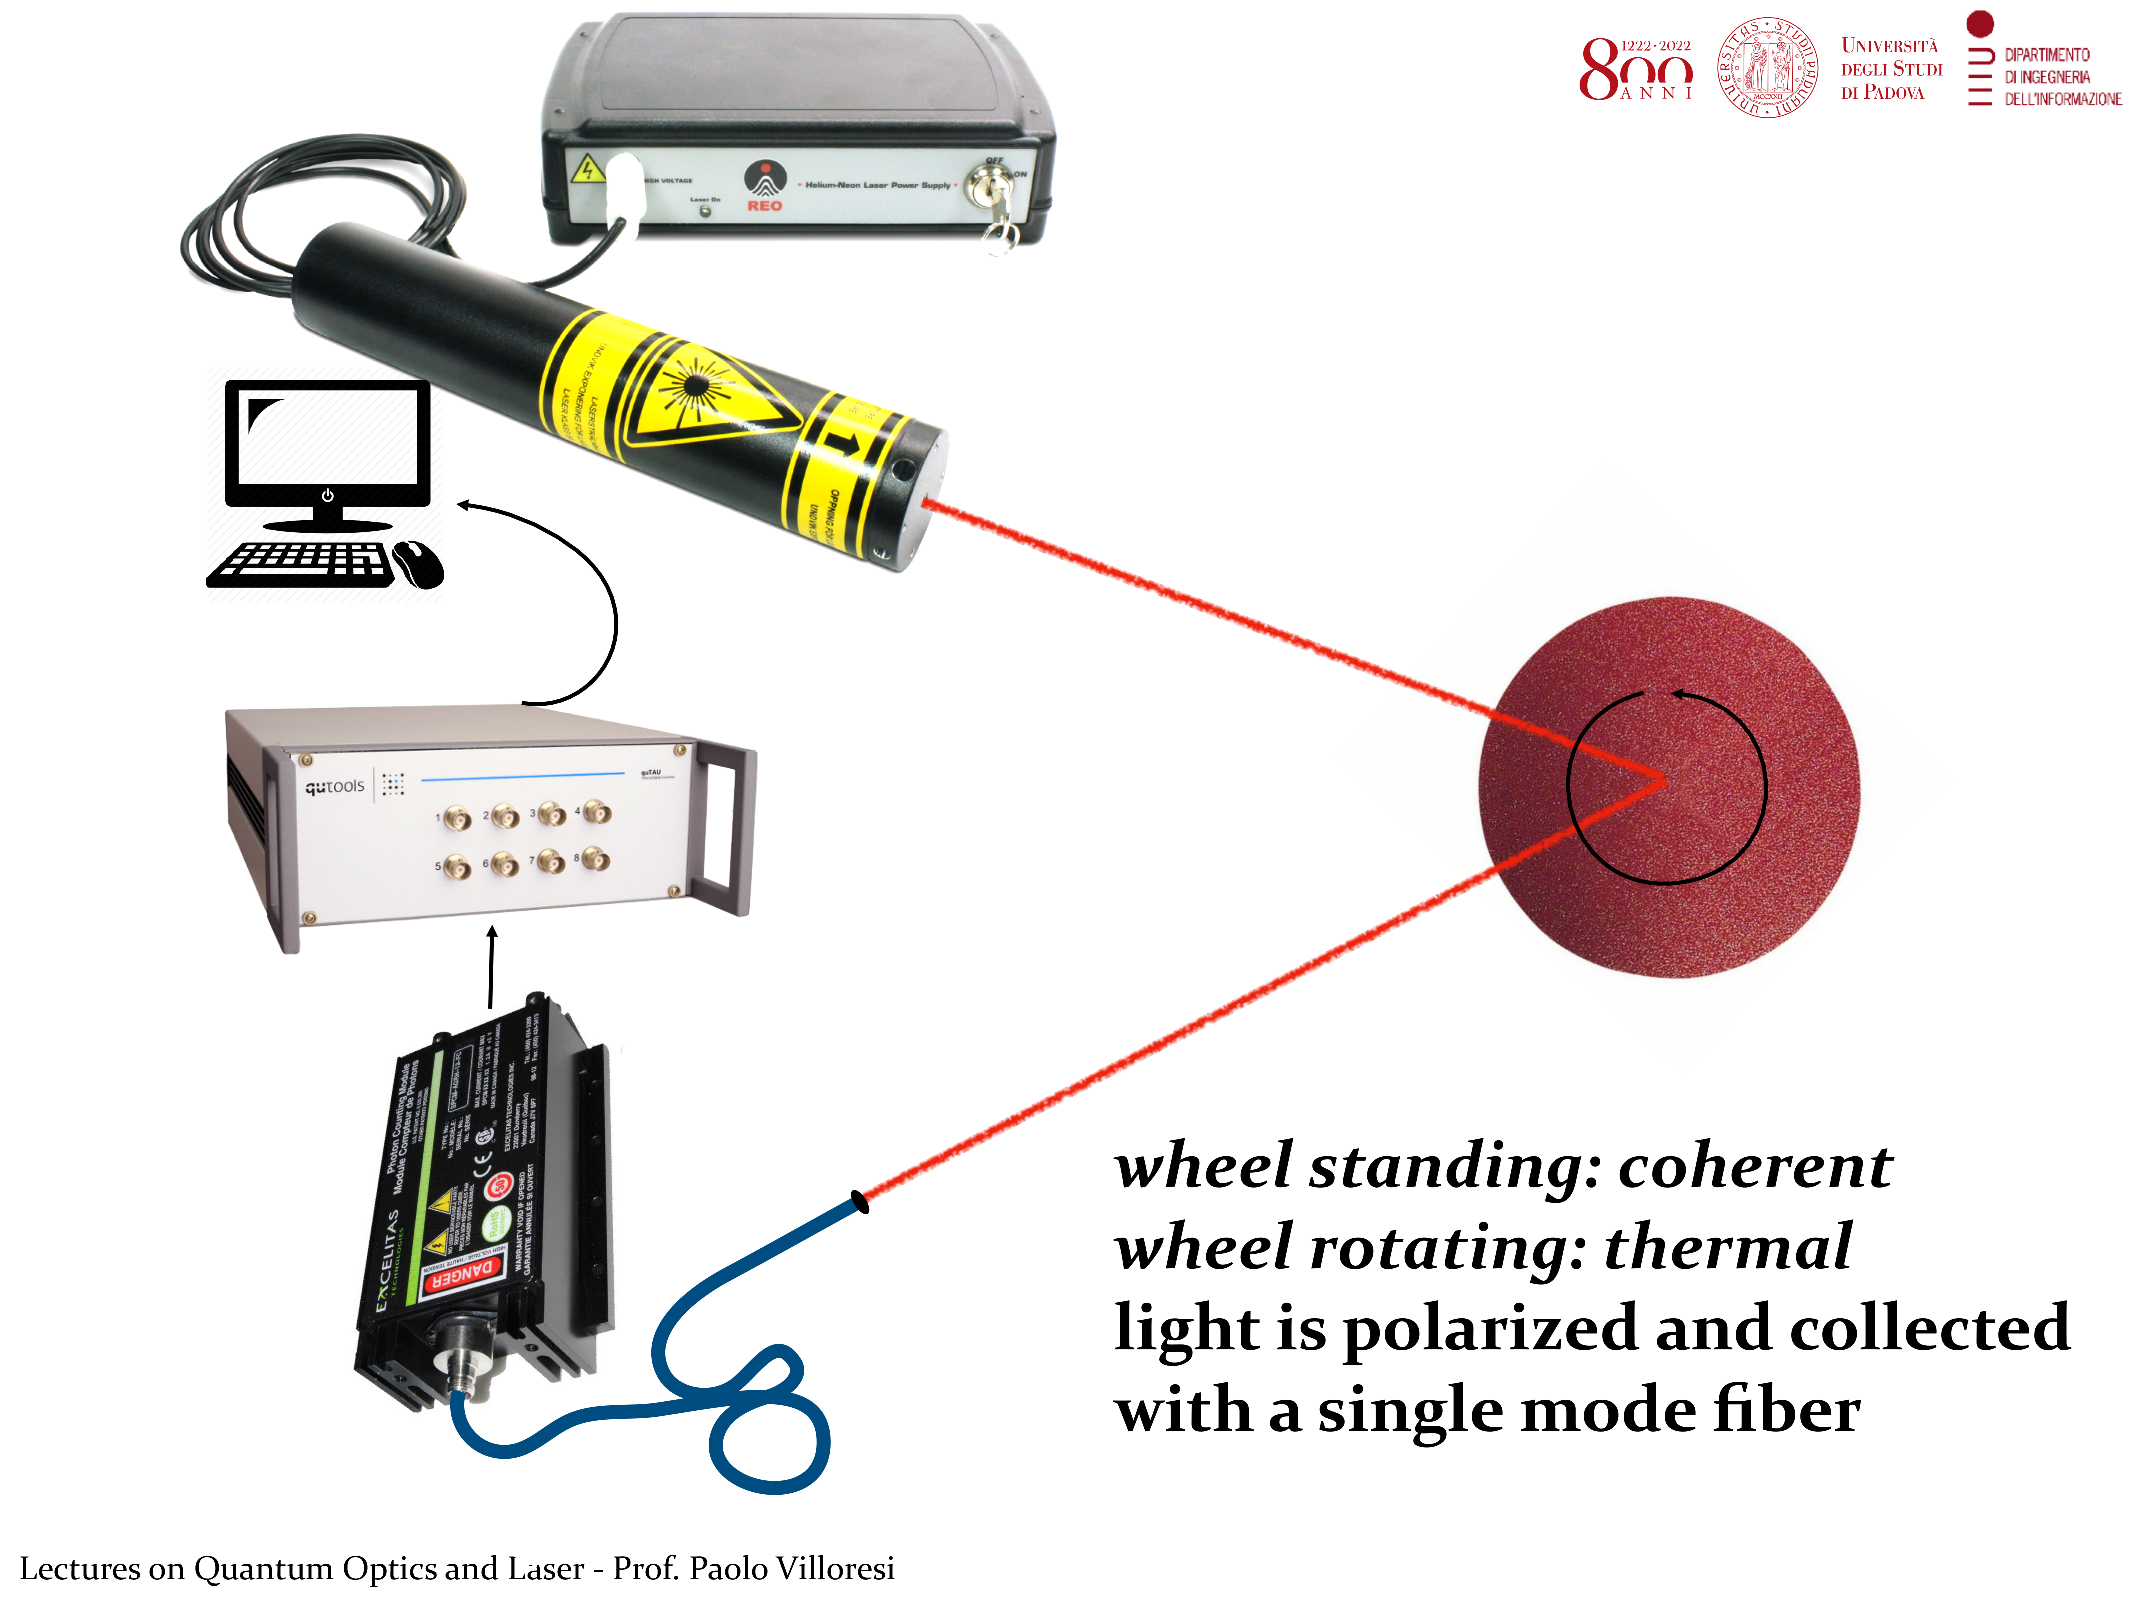
\includegraphics[width=0.6\textwidth]{images/setup.pdf}
    \caption{Setup for the Arecchi experiment.}
    \label{fig:setup}    
\end{figure}

The objective of the experience is to take an interval of time $T$ (a good one is around $15\mu s$) and count how many photons reached the detector (\emph{occurrences}) in about $2s$ of data collection. The histogram of the occurrences with respect to the number of photons in the time bin $T$ should follow a statistic probability in the two cases:
\begin{itemize}
\item \emph{still wheel}: a \emph{Poisson} distribution $\mathscr{P}(\lambda)=\dfrac{\lambda^n exp(-\lambda)}{n!}$  with $n=0,1,2...$;
\item \emph{spinning wheel}: a \emph{Bose-Einstein} distribution $BE (\lambda)=\dfrac{1}{\lambda+1}\left(\dfrac{\lambda}{\lambda +1}\right)^n$  with $n=0,1,2...$
\end{itemize}
where $\lambda$ represents the mean arrival of photons in $T$.